\documentclass[]{article}

\usepackage{caption}
\usepackage{graphicx, subfig}
\usepackage{listings}
\usepackage[namelimits]{amsmath} 
\usepackage{fontspec}
\usepackage{amsmath}
\usepackage{amssymb}                      
\usepackage{mathrsfs}  
\usepackage{amsfonts}   
\setmainfont[Mapping=tex-text]{KaiTi}
\usepackage{fullpage}
\usepackage{amsthm}
\usepackage{fancyhdr}
\usepackage{algorithm}
\usepackage{algorithmic}
\usepackage{bm}
\usepackage{ctex}
\usepackage{txfonts}
\usepackage{tikz}
\usetikzlibrary{shapes.geometric, arrows}


%opening
\title{统计机器学习 课后作业9}
\author{陈劭涵 17300180049}



\newcommand{\tm}{\fontspec{Times New Roman}}


\begin{document}
	
\maketitle


\section{问题 1.1}
\begin{flushleft}
解:
\end{flushleft}
$Y=(Y_1,Y_2,...,Y_m)^T=(\alpha_1^T,\alpha_2^T,...,\alpha_m^T)^T X=\begin{pmatrix}
	\alpha_{11}  & \alpha_{12}&... & \alpha_{1m}\\
	\alpha_{21}  & \alpha_{22}&... & \alpha_{2m}\\
	\vdots  & \vdots&\ddots & \vdots \\
	\alpha_{m1} &\alpha_{m2}&  ... & \alpha_{mm}\\
\end{pmatrix}$\\\\
令$A=\begin{pmatrix}
	\alpha_{11}  & \alpha_{12}&... & \alpha_{1m}\\
	\alpha_{21}  & \alpha_{22}&... & \alpha_{2m}\\
	\vdots  & \vdots&\ddots & \vdots \\
	\alpha_{m1} &\alpha_{m2}&  ... & \alpha_{mm}\\
\end{pmatrix}$\\\\
则$X=A^TY=\begin{pmatrix}
	\alpha_{11}  & \alpha_{12}&... & \alpha_{1m}\\
	\alpha_{21}  & \alpha_{22}&... & \alpha_{2m}\\
	\vdots  & \vdots&\ddots & \vdots \\
	\alpha_{m1} &\alpha_{m2}&  ... & \alpha_{mm}\\
\end{pmatrix}^TY$\\\\
$\therefore X_i=\sum_{k=1}^{m}\alpha_{ki}Y_k$\\\\
则$\sigma_{ii}=Var(X_i)=Var(\sum_{k=1}^{m}\alpha_{ki}Y_k)=\sum_{k=1}^{m}\alpha_{ki}^2Var(Y_k)=\sum_{k=1}^{m}\alpha_{ki}^2\lambda_k$\\\\
$\therefore \sum_{k=1}^{m}\rho^2(Y_K,X_i)=\sum_{k=1}^{m}\frac{\lambda_k\alpha_{ki}^2}{\sigma_{ii}}=\frac{\sum_{k=1}^{m}\lambda_k\alpha_{ki}^2}{\sigma_{ii}}=1$\\\\

\section{问题 1.2}
\begin{flushleft}
	解:
\end{flushleft}
对样本阵X进行标准化:\\\\
$\bar{x_i}=\frac{\sum_{j=1}^{n}x_{ij}}{n},\ s_{ii}=\frac{\sum_{j=1}^{n}(x_{ij}-\bar{x_i})^2}{n-1}$\\\\
$x^*_{ij}=\frac{x_{ij}-\bar{x_i}}{\sqrt{s_{ii}}}$\\\\
$\therefore$标准化后的矩阵为 $X^*=\begin{pmatrix}
	-\frac{\sqrt{5}}{2}&-\frac{\sqrt{5}}{4}&-\frac{\sqrt{5}}{4}&0&\frac{\sqrt{5}}{4}&\frac{3\sqrt{5}}{4}\\
	-\frac{3}{2}&-\frac{1}{2}&0&0&\frac{1}{2}&\frac{3}{2}\\
\end{pmatrix}$\\\\
$\therefore S=\begin{pmatrix}
1&\frac{17\sqrt{5}}{40}\\
\frac{17\sqrt{5}}{40}&1\\
\end{pmatrix}$
进行特征值分解得:\\\\
$\lambda_1=\frac{40+17\sqrt{5}}{40}$\\\\
$\alpha_1=(\frac{1}{\sqrt{2}},\frac{1}{\sqrt{2}})^T$\\\\
$\lambda_1=\frac{40-17\sqrt{5}}{40}$\\\\
$\alpha_2=(\frac{1}{\sqrt{2}},-\frac{1}{\sqrt{2}})^T$\\\\
$\Rightarrow y_1=\frac{1}{\sqrt{2}}x_1+\frac{1}{\sqrt{2}}x_2$, $y_2=\frac{1}{\sqrt{2}}x_1-\frac{1}{\sqrt{2}}x_2$\\\\
$\because \frac{\lambda_1}{\lambda_1+\lambda_2}=0.975$\\\\
$\therefore$主成分$y_1$包含了样本的相当大部分信息内容
\section{问题 1.3}
\begin{flushleft}
	解:
\end{flushleft}
若样本协方差矩阵S是总体协方差矩阵方差$\Sigma$的无偏估计,则:\\\\
$\forall i,j,\  E(S_{ij})=\Sigma_{ij}$\\\\
$S_{ij}=\frac{1}{n-1}\sum_{k=1}^{n}(x_{ik}-\bar{x_i})(x_{jk}-\bar{x_j})$\\\\
$=\frac{1}{n-1}\sum_{k=1}^{n}(x_{ik}-\mu_i+\mu_i-\bar{x_i})(x_{jk}-\mu_j+\mu_j-\bar{x_j})$\\\\
$=\frac{1}{n-1}\sum_{k=1}^{n}\left[(x_{ik}-\mu_i)(x_{jk}-\mu_j)+(x_{ik}-\mu_i)(\mu_j-\bar{x_j})+(\mu_i-\bar{x_i})(x_{jk}-\mu_j)+(\mu_i-\bar{x_i})(\mu_j-\bar{x_j})\right]$\\\\
$\therefore E(S_{ij})=E\sum_{k=1}^{n}(x_{ik}-\mu_i)(x_{jk}-\mu_j)+E\sum_{k=1}^{n}(\mu_j-\bar{x_j})(x_ik-\mu_i)+E\sum_{k=1}^{n}(\mu_i-\bar{x_i})(x_{jk}-\mu_j)+E\sum_{k=1}^{n}(\mu_i-\bar{x_i})(\mu_j-\bar{x_j})$\\\\
$\because E\sum_{k=1}^{n}(x_{ik}-\mu_i)(x_{jk}-\mu_j)=\sum_{k=1}^{n}E(x_{ik}-\mu_i)(x_{jk}-\mu_j)=\sum_{k=1}^{n}Cov(X_i,X_j)=n\Sigma_{ij}$\\\\
$E\sum_{k=1}^{n}(\mu_j-\bar{x_j})(x_ik-\mu_i)=\frac{-1}{n}\sum_{k=1}^{n}\sum_{m=1}^{n}E(x_{jm}-\mu_j)(x_{ik}-\mu_i)=\frac{-1}{n}\sum_{k=1}^{n}E(x_{jk}-\mu_j)(x_ik-\mu_i)=-\Sigma_{ij}$\\\\
$E\sum_{k=1}^{n}(\mu_i-\bar{x_i})(x_{jk}-\mu_j)=\frac{-1}{n}\sum_{k=1}^{n}\sum_{m=1}^{n}E(x_{im}-\mu_i)(x_{jk}-\mu_j)=\frac{-1}{n}\sum_{k=1}^{n}E(x_{ik}-\mu_i)(x_jk-\mu_j)=-\Sigma_{ij}$\\\\
$E\sum_{k=1}^{n}(\mu_i-\bar{x_i})(\mu_j-\bar{x_j})=\frac{1}{n}\sum_{k=1}^{n}\sum_{m=1}^{n}E(x_{im}-\mu_i)(x_{jk}-\mu_j)=\Sigma_{ij}$\\\\
$\therefore E(S_{ij})=E\sum_{k=1}^{n}(x_{ik}-\mu_i)(x_{jk}-\mu_j)+E\sum_{k=1}^{n}(\mu_j-\bar{x_j})(x_ik-\mu_i)+E\sum_{k=1}^{n}(\mu_i-\bar{x_i})(x_{jk}-\mu_j)+E\sum_{k=1}^{n}(\mu_i-\bar{x_i})(\mu_j-\bar{x_j})$\\\\
$=\frac{1}{n-1}((n-1)\Sigma_{ij})=\Sigma_{ij}$\\\\

\section{问题 1.4}
\begin{flushleft}
	解:
\end{flushleft}
主成分问题的求解本质上是将样本点投影到一个超平面上,使得样本点到超平面的距离足够近(最近重构性),即样本点与其投影的总距离最小化\\\\
故该问题可以根据如下过程转化:\\\\
设$X$是数据规范化样本矩阵,假设取k个主成分,那么我们要把样本点投影到k维的向量子空间上. 假设$A$是一个k维的正交矩阵,即$A^TA=I_k$,我们可以把$A=(A_1,A_2,...,A_k)\in \mathbb{R^{m\times k}}$视作一组$\mathbb{R}$的一个k维子空间的标准正交基\\\\
对于样本点$X_i\in \mathbb{R}$,将其在子空间超平面上的投影表示为$\tilde{X}$\\\\
则根据投影性质:$A_{1\leq p\leq k}^T(X_i-\tilde{X})=0$\\\\
$\therefore A^T(X_i-\tilde{X})=0 \Rightarrow A^TX_i=A^T\tilde{X}$\\\\
$\therefore \tilde{X}=AA^TX_i$\\\\
则样本点与投影的距离和为$d=\sum_{i=1}^{n}\vert\vert X_i-\tilde{X}\vert\vert^2=\sum_{i=1}^{n}\vert\vert X_i-AA^TX_i\vert\vert^2=\sum_{i=1}^{n}\sum_{j=1}^{m}\vert X-AA^TX\vert_{jj}$\\\\
$=\vert\vert X-AA^TX\vert\vert_F^2$\\\\
所以主成分问题等价于求解:\\\\
$min\ \vert\vert X-AA^TX\vert\vert_F$\\
$s.t. \ A^TA=I_k\ ,\ A\in \mathbb{R}^{m\times k}$
$\because$  $A$和$A^T$都是可逆矩阵\\\\
$\therefore$ 根据矩阵秩的性质:\\
$rank(A)=rank(A^T)$\\
$rank(A^TA)=rank(A)=rank(AA^T)$\\
$\therefore rank(A)=rank(A^T)=rank(AA^T)=k$\\\\
又根据矩阵秩的性质:\\
$rank(AA^TX)\leq min(rank(AA^T),rank(X))$\\
$\because rank(AA^T)=k$\\
$\therefore rank(AA^TX)\leq k$\\\\
我们令$L=AA^TX$,则问题便转化为\\\\
$min\ \vert\vert X-L\vert\vert_F$\\
$s.t. \ rank(L)\leq k$\\\\
则命题得证

\section{问题 2}
\begin{flushleft}
	解:
\end{flushleft}
1、读入数据
\begin{lstlisting}
	library("xlsx")
	data=read.xlsx("D:/大数据学院文件资料/2020秋课程/机器学习/assignment
	/homework9/NBA数据分析降维/NBA.xlsx",1,encoding = "UTF-8")
\end{lstlisting}
2、主成分分析\\\\
由于数据表中的投篮命中率等几项中,存在\%等字符,不方便进行直接使用,需要进行一定修正
\begin{lstlisting}
	# 做修正
	data$投篮率 <- as.numeric(gsub("\\%", "", data$投篮率))/100 
	data$三分投球率 <- as.numeric(gsub("\\%", "", data$三分投球率))/100 
	data$罚球率 <- as.numeric(gsub("\\%", "", data$罚球率))/100
	train_data=data
	train_data[2:18]=scale(data[2:18])
	pca=princomp(train_data[,2:(ncol(train_data)-1)],cor=FALSE)
	pca
	# 崖底碎石图
	screeplot(pca,type="lines",cex.lab=1,main="崖底碎石图")
\end{lstlisting}
主成分分析内容如下:
\begin{lstlisting}
	> pca
	Call:
	princomp(x = train_data[, 2:(ncol(train_data) - 1)], cor = FALSE)
	
	Standard deviations:
	Comp.1     Comp.2     Comp.3     Comp.4     Comp.5     Comp.6     Comp.7     
	3.25955118 1.32224439 1.09924743 0.92902888 0.81337097 0.77461728 0.66182260 
	Comp.8	    Comp.9    Comp.10  
	0.57464925 0.41047089 0.33385999 
	Comp.11    Comp.12    Comp.13    Comp.14    Comp.15    Comp.16    Comp.17 
	0.30978107 0.25997482 0.19222853 0.15187864 0.08545811 0.07330772 0.05079972 
	
	17  variables and  2448 observations.
\end{lstlisting}
崖底碎石图如下:\\\\
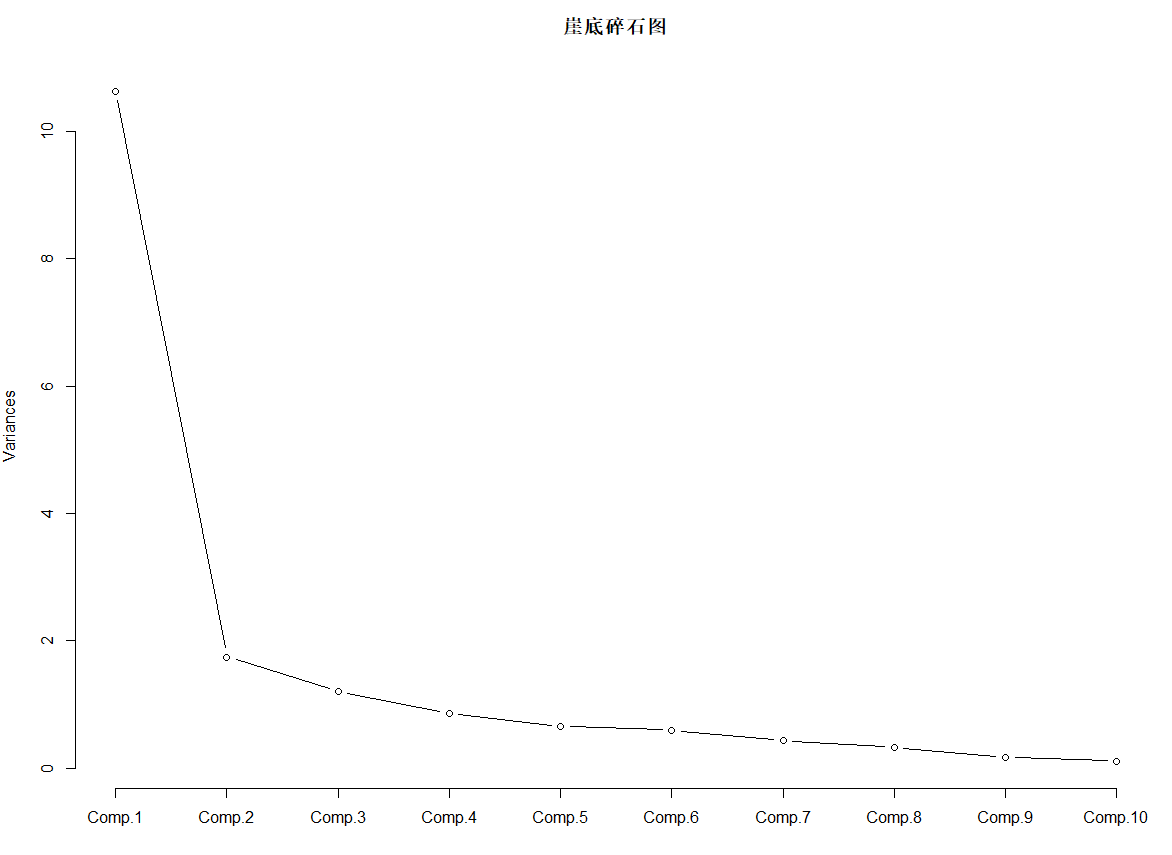
\includegraphics[width=.9\textwidth]{D:/大数据学院文件资料/2020秋课程/机器学习/homework/hw9/util/崖底碎石图.png}\\\\
由principle函数返回结果以及崖底碎石图,我们看到主成分数量大于一之后特征值大幅度下降,除了第一个主成分,其余的方差贡献率都比较低,所以我们就选取一个主成分\\
如果要求总体方差贡献率超过80\%,则我们也可以选取前三个主成分\\\\
3、根据任务2的结果,计算每一位球员的主成分得分\\\\
在本题中我们使用一个主成分来进行分析
\begin{lstlisting}
	pca_value=numeric(0)
	data1=data
	data1[2:18]=scale(data1[2:18])
	# 计算所有球员的主成分得分
	for(i in 1:nrow(data1)){
		pca_value=c(pca_value,as.matrix(data1[i,2:(ncol(data1)-1)])
		%*%as.matrix(pca$loadings[,1]
		))
	}
	head(pca_value)
	# 解读某几位球员的主成分得分
	value1=as.matrix(data1[data1$球员=='勒布朗-詹姆斯',2:(ncol(data1)-1)])
	%*%as.matrix(pca$loadings[,1])
	value2=as.matrix(data1[data1$球员=='科比-布莱恩特',2:(ncol(data1)-1)])
	%*%as.matrix(pca$loadings[,1])
	value3=as.matrix(data1[data1$球员=='卡尔-马龙',2:(ncol(data1)-1)])
	%*%as.matrix(pca$loadings[,1])
	value4=as.matrix(data1[data1$球员=='斯蒂芬-库里',2:(ncol(data1)-1)])
	%*%as.matrix(pca$loadings[,1])
	value5=as.matrix(data1[data1$球员=='保罗-乔治',2:(ncol(data1)-1)])
	%*%as.matrix(pca$loadings[,1])
	value6=as.matrix(data1[data1$球员=='凯文-乐福',2:(ncol(data1)-1)])
	%*%as.matrix(pca$loadings[,1])
	value7=as.matrix(data1[data1$球员=='艾德-戴维斯',2:(ncol(data1)-1)])
	%*%as.matrix(pca$loadings[,1])
	value8=as.matrix(data1[data1$球员=='汤姆-里克尔',2:(ncol(data1)-1)])
	%*%as.matrix(pca$loadings[,1])
	show=cbind(c('勒布朗-詹姆斯','科比-布莱恩特','卡尔-马龙','斯蒂芬-库里',
	'保罗-乔治','凯文-乐福','艾德-戴维斯','汤姆-里克尔')
	,rbind(value1,value2,value3,value4,value5,value6,value7,value8))
	show_value=as.data.frame(row.names=c('d','d'),col.names=c('a','d'),show)
	colnames(show_value) = c("球员名字","主成分得分")
	show_value
\end{lstlisting}
球员主成分得分:
\begin{lstlisting}
	> head(pca_value)
	[1] 34.35805 24.75592 18.30285 26.51568 24.23799 25.77510
\end{lstlisting}
挑选某几位球员进行解读:
\begin{lstlisting}
	> show_value
	球员名字         主成分得分
	1 勒布朗-詹姆斯   34.3580495957784
	2 科比-布莱恩特      26.5156789029
	3     卡尔-马龙   21.2006035760464
	4   斯蒂芬-库里   13.4251625700673
	5     保罗-乔治   8.16961345311563
	6     凯文-乐福   4.60012891064624
	7   艾德-戴维斯 -0.803009875406259
	8   汤姆-里克尔  -2.02865087422127
\end{lstlisting}
我们从数据表的各个部分中分别挑选了几位球员作为代表,得到如上的主成分得分案例表\\\\
我们结合第一主成分参数表进行解,第一主成分参数表如下:
\begin{lstlisting}
	> pca$loadings[,1]
	出场数 上场总时间.min.          投篮率 
	0.28222457      0.29794775      0.05886760 
	命中次数        出手次数      三分投球率 
	0.29316496      0.29365700      0.06570046 
	三分命中次数    三分出手次数          罚球率 
	0.19802884      0.20526898      0.08702051 
	罚球命中次数    罚球出手次数          篮板数 
	0.28498994      0.28402349      0.25666021 
	助攻次数        抢断次数        盖帽次数 
	0.26526333      0.26630866      0.20583656 
	失误次数        犯规次数 
	0.26922807      0.28069657 
\end{lstlisting}
结合如上的案例表和参数表我们可以看到,数据表中的所有特征与第一主成分均呈正相关关系. 对主成分影响较大的几个特征是上场时间,命中次数和出手次数,参数分别为0.298, 0.294和0.293, 意味着上场时间每增加一分钟,命中次数和出手次数每增加一,主成分得分就分别增加0.298, 0.294和0.293.
对主成分影响较低的几个特征是投篮率,三分投球率和罚球率,其参数均未超过0.1,远小于其他特征.\\\\
此外,我们对这几名球员的选择其实是根据其生涯总得分的排名来选择的,从这几个球员中可以看到,生涯总得分越高的球员,主成分得分越高。可以看到勒布朗-詹姆斯作为球星和球队核心的主成分得分和总得分最高,汤姆-里克尔作为角色球员的主成分得分和总得分最低,不难看出生涯总得分越高,主成分得分越高的球员,综合能力越强。这也与勒布朗詹姆斯常年闯进季后赛和总决赛,季后赛上场时间多,出手和得分多,综合能力强的情况符合。此外列表中主成分得分的排名也与我们所认识的球员能力和生涯表现总体上相匹配,说明主成分分析对NBA季后赛数据有较好的建模效果\\\\
4、对NBA球员进行K-means聚类,并对结果进行解读\\\\
首先预估一下要聚类的类别数
\begin{lstlisting}
	# 评估类别数
	class_num=numeric(15)
	for(i in 1:15){
		clusters=kmeans(data1[,2:(ncol(data1)-1)],centers=i)
		class_num[i]=max(clusters$withinss)
	}
	plot(class_num,xlab="聚类的类别数",ylab="clusters$withinss类别内距离度量"
	,main="类别内距离~聚类类别数",type='o')

\end{lstlisting}
评估结果如下:\\\\
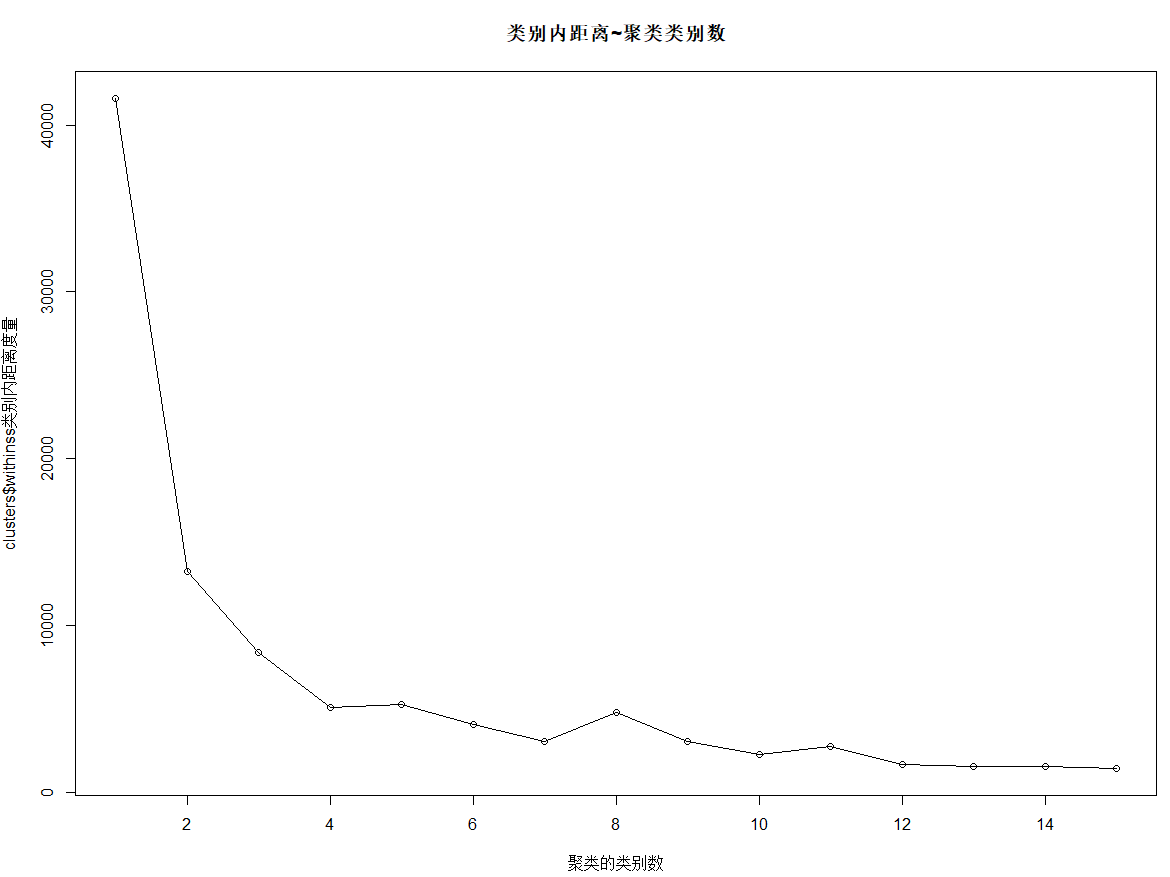
\includegraphics[width=.9\textwidth]{D:/大数据学院文件资料/2020秋课程/机器学习/homework/hw9/util/聚类评估结果.png}\\\\
从上图中我们可以观察到,在聚类的类别数量大于等于4或5的时候,类别内距离趋于较为稳定的低值,虽然有些许波动但没有太大影响,于是我们选取聚类类别数=4,进行聚类如下:\\\\
\begin{lstlisting}
	# 进行聚类
	clusters=kmeans(data1[,2:(ncol(data1)-1)],centers=4)
	cluster_res=cbind(data1[2:18],clusters$cluster)
	c_res=aggregate(cluster_res,by=list(clusters$cluster),mean)
	colnames(c_res)[1]="聚类分组编号"
	head(c_res)
\end{lstlisting}
聚类结果如下:\\\\
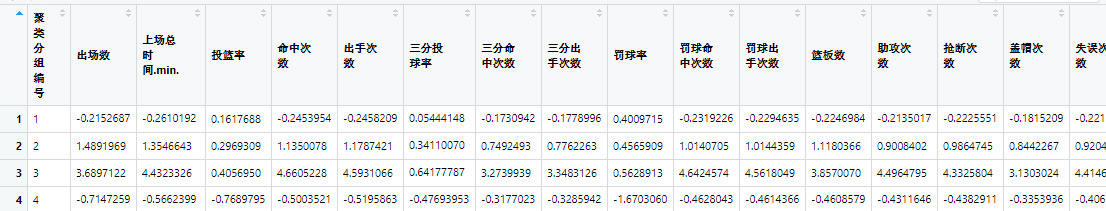
\includegraphics[width=1.0\textwidth]{D:/大数据学院文件资料/2020秋课程/机器学习/homework/hw9/util/聚类结果.png}\\\\
从如上聚类结果我们可以进行解读:\\\\
1、可以看到分组编号为3的球员组,在出场时间,投篮率,命中次数,出手次数和三分球,篮板和助攻等方面的数值都是最高的,因此可以认为这组球员通常是球队的核心球员和首发球员,因此他们的上场时间多,球权和出手权较多,使得对应的数值都较高。通常球队的核心是综合能力以及得分能力强的球员,如乔丹、詹姆斯、科比、奥拉朱旺等,所以在这些特征上的表现都较高。例外如马努吉诺比利,虽然是球队的替补球员,但是是球队核心之一,也属于这一组\\\\
2、可以看到分组编号为2的球员组,在出场时间,投篮率,命中次数,出手次数和三分球,篮板和助攻等方面的数值都是次高的,虽然少于第3组,但是远高于剩余两组,因此可以认为这组球员通常是球队的功能性球员,强力替补球员,轮换球员等,如卡隆-巴特勒,马特-巴恩斯等。一些缺少攻击性的球队首发球员也属于这一类\\\\
3、可以看到分组编号为1的球员组在出场时间,投篮率,命中次数,出手次数和三分球,篮板和助攻等方面的数值都是较低的,这类球员可能是功能型球员,能力一般的角色球员,球队新秀等,上场时间较少,能力一般,所以各特征数值也较低\\\\
4、可以看到分组编号为4的球员在出场时间,投篮率,命中次数,出手次数和三分球,篮板和助攻等方面的数值都是较低的,这类球员一般为角色球员,边缘球员,通常很少在季后赛上场,上场时间非常少,能力较差,所以各特征数值也较低\\\\
总体来说,K-means聚类较好得将球员分成了各不相同的四类球员\\\\

\section{问题 3}
代码如下:
\begin{lstlisting}
	PCA<-function(Dat,max.k){
		X=as.matrix(Dat) 
		R=1/(nrow(X)-1)*t(X)%*%X 
		lambda=eigen(R)$values[1:max.k] 
		para=eigen(R)$vectors[,1:max.k] 
		return(list(sdev=sqrt(lambda),paramatrix=para))
	}
	PCA_res=PCA(Dat=data1[,2:(ncol(data1)-1)],max.k=10)
	PCA_res
	screeplot(PCA_res,type="lines",cex.lab=1,main="PCA函数崖底碎石图")
\end{lstlisting}
测试结果如下:\\\\
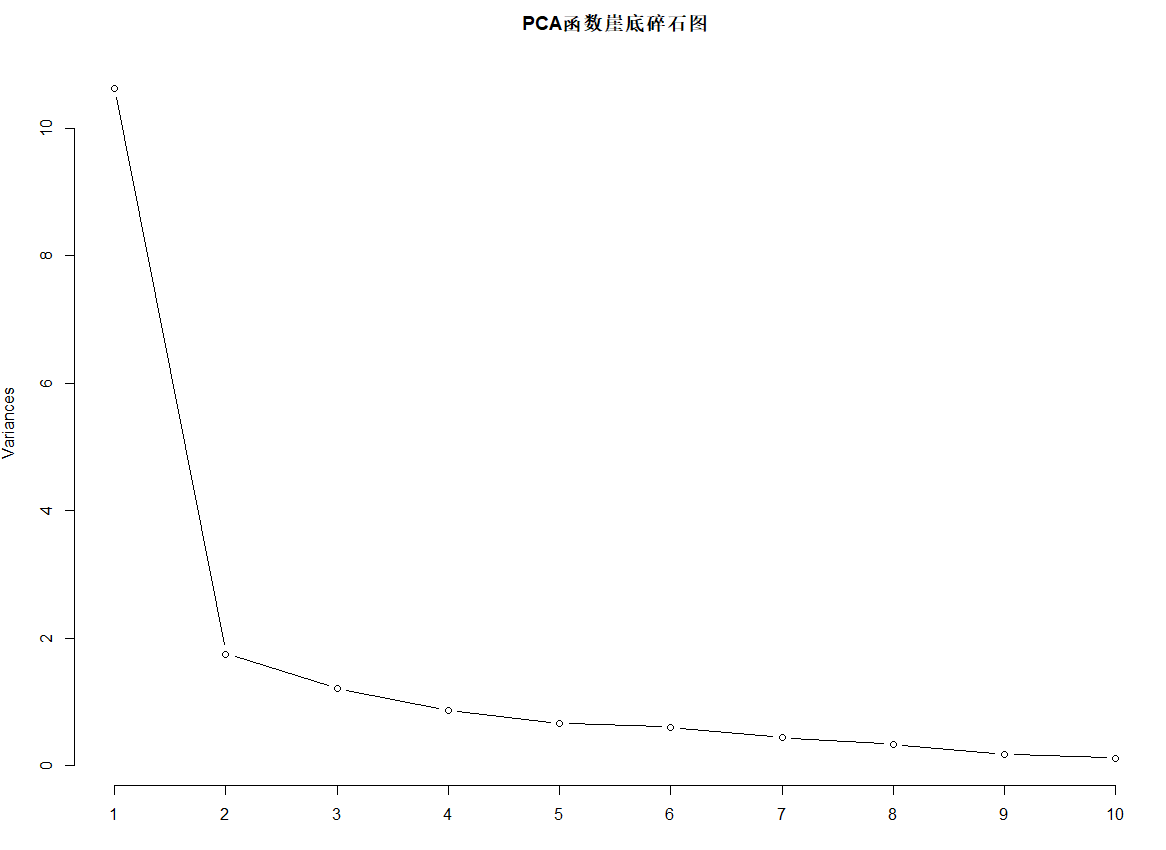
\includegraphics[width=1.0\textwidth]{D:/大数据学院文件资料/2020秋课程/机器学习/homework/hw9/util/崖底碎石图测试.png}\\\\
\end{document}
